% Please use the skeleton file you have received in the
% invitation-to-submit email, where your data are already
% filled in. Otherwise please make sure you insert your
% data according to the instructions in PoSauthmanual.pdf

\documentclass{PoS}

%\usepackage{hyperref}
%%\hypersetup{colorlinks=false}
%
%\usepackage[backend=biber,
%hyperref=true,
% url=true, 
%    doi=false,
%    eprint=true]{biblatex}
%%\usepackage{atlasbiblatex}
%\addbibresource{bib/ATLAS.bib}
%\addbibresource{bib/CMS.bib}
%\addbibresource{bib/ConfNotes.bib}
%\addbibresource{bib/PubNotes.bib}

%
%\hypersetup{
%    colorlinks=true,
%}
%\bibliographystyle{JHEP}
%\bibliography{bib/ATLAS.bib}



          
\title{Searches for high-mass resonances decaying to pair of bosons using the ATLAS detector}

\ShortTitle{Searches for high-mass resonances}

\author{\speaker{Kirill Grevtsov}, {on behalf of the ATLAS collaboration}\\%\thanks{A footnote may follow.}\\
        Deutsches Elektronen-Synchrotron, DESY\\
        E-mail: \email{kirill.grevtsov@cern.ch}}

%\author{Another Author\\
%        Affiliation\\
%        E-mail: \email{...}}
%http://www.ichep2018.org/03_abstract/s31.html#Proceedings
% There is a page limit:
% 
%  - Parallel talk: 4 pages for <20 min, including the title and reference 

\abstract{Several theories beyond the Standard Model predict the existence of new heavy particles decaying into pairs of gauge bosons. In this proceedings the latest ATLAS results on searches for resonances decaying into pairs of $W$ or $Z$ bosons or photon  based on datasets of 36  and 80 fb$^{-1}$ of $pp$ collision data collected at 13 TeV will be discussed.
}

\FullConference{ICHEP 2018, International Conference on High Energy Physics\\
		4-11 July 2018\\
		Seoul, South Korea}



\begin{document}



\section{Introduction}

The discovery of a Higgs-like particle announced by the ATLAS and CMS Collaborations in 2012 \cite{HIGG-2012-27,CMS-HIG-12-028} has been an important milestone in the understanding of the mechanism of electroweak (EW) symmetry breaking. %[3-5].
%3. F. Englert, R. Brout, Broken symmetry and the mass of gauge vector mesons. Phys. Rev. Lett. 13, 321 (1964). https://doi.org/10.1103/ PhysRevLett.13.321
%4. P.W. Higgs, Broken symmetries and the masses of gauge bosons. Phys. Rev. Lett. 13, 508 (1964). https://doi.org/10.1103/ PhysRevLett.13.508
%5. G.S. Guralnik, C.R. Hagen, T.W.B. Kibble, Global conservation laws and massless particles. Phys. Rev. Lett. 13, 585 (1964). https:// doi.org/10.1103/PhysRevLett.13.585
Next step is to figure out whether this particle is the only one or if it is part of an extended Higgs sector as predicted by several extensions of the Standard Model (SM): composite Higgs models, heavy vector triplets and models with warped extra dimensions
%Diboson vector and tensor resonances are also predicted in several other extensions to the SM, such as in composite Higgs mod- els [9, 10] and models with warped extra dimensions [11?14].


In these proceedings a collection of different results is presented.
A search for additional heavy resonances in diboson final states presented for several channels: leptonic decays of $W$ and $Z$ boson pairs described in Section~\ref{sec:WW} and \ref{sec:ZZ} for 36fb$^{-1}$; fully hadronic decays of $VV$ described in Section~\ref{sec:VV} using 80 fb$^{-1}$ dataset; results of searches for photon and hadronicaly decaying $Z,W$ or $H$ bosons are presented in Section~\ref{sec:gV}. The brief overview of searches are summarised in Section~\ref{sec:sum}.

%\newpage

\section{$WW\rightarrow e\nu \mu \nu$ decays}
\label{sec:WW}
The search for neutral heavy resonance $H$ decaying to $WW$ with final state $e\nu \mu \nu$ is described in detail in~\cite{HIGG-2016-31}. Search is performed for production via the quark-antiquark annihilation ($q\bar{q}A$), vector-boson fusion (VBF) or gluon-gluon fusion ($ggF$) process covering mass range from 200 GeV up to 5 TeV for various benchmark models: a Higgs-like scalar in different width scenarios (NWA-LWA, 0-15\%$m_X$), a two-Higgs-doublet model (2HDM), a heavy vector triplet model (HVT), a warped extra dimensions model ($G_{KK}$) and the Georgi-Machacek (GM) model.

Analysis looking into opposite sign different flavour leptons, categorising event into three signal regions (SR), two VBF enriched and one targeting $ggF/q\bar{q}A$. For each signal region corresponding control region (CR) defined to estimate normalisations for main backgrounds ($t\bar{t}$ and non-resonant $WW$). 
Shapes of main backgrounds are taken from simulation and normalised using dedicated CRs, while $W$+jets background taken from data-drive estimates.
Due to the presence of large missing energy, discriminant variable is transverse mass ($m_T$), fitted simultaneously in SRs and CRs. 
%Plots shows binned transverse mass distribution for two signal regions, for data and background predictions. 
%Data fitted simultaneously in all the SRs and the CRs - no excess over the background prediction is observed
As no excess over the background prediction is observed, upper limits at 95\% CL$_s$ on $\sigma_H \times B(H\rightarrow WW)$ are set for $ggF$($VBF$) in range 0.2 - 4(3) TeV. Limit translated to exclusion contours in the 2HDM in the plane of $tan \beta$ versus $cos(\beta-\alpha)$.
 Values above 6.4 pb (1.3 pb) at $m_H$ = 200 GeV and above 0.008 pb (0.006 pb) at 4 (3) TeV are excluded at 95\% CL by the quasi-inclusive $ggF$(VBF) NWA analysis.
% For the LWA 15\% case, the upper exclusion limit ranges between 5.2 pb (1.3 pb) at m H = 200 GeV and 0.02 pb (0.006 pb) at 4 (3) TeV for the $ggF$(VBF) signals.
Limits are set for signal widths of 5, 10 and 15\% and are compatible with the NWA one.
The current sensitivity is not sufficient to exclude GM signal with masses between 200 GeV and 1 TeV.
Heavy vector triplet signals below about 1.3 TeV are excluded at 95\% CL. 
The observed limits exclude a KK graviton signal lighter than 1.1 TeV (750 GeV) with the higher (lower) coupling, while the current sensitivity is not sufficient to exclude the ELM spin-2 VBF signal. 

\section{$ZZ\rightarrow \ell^+\ell^-\ell^+\ell^-$ and $\ell^+\ell^-\nu\bar{\nu}$ decays} %l+l?l+l?
\label{sec:ZZ}
Searches for a heavy resonance decaying into two SM $Z$ bosons performed in four lepton and two lepton two neutrino channels~\cite{HIGG-2016-19}, with similar strategies as discussed in Section~\ref{sec:WW}. Search performed in range from 200 GeV up to 1.4 TeV for narrow width signals and up to 1 TeV for large width hypothesis in search for scalar. Search for graviton done in range up to 2 TeV.

Analysis selecting two same-flavour, opposite-sign lepton pairs in $4\ell$ channel and one pair with 120 GeV cut on missing energy of escaping neutrinos in $2\ell2\nu$.
Events are classified into categories: VBF and three $ggF$ for each of the lepton pair flavour.
Four lepton mass ($m_{4\ell}$) and transverse mass ($m_T$) used as discriminant variables in $4\ell$ and $2\ell2\nu$ channels correspondingly.
Signal described as CrystalBall+Gaussian (moment-morphing) used to model signal in $4\ell$ ($2\ell2\nu$) channel. Both channels uses same strategy for large width and accounting for interference between signal and non-resonant $ZZ$ and with 125 GeV Higgs to $ZZ$.
Non resonant $ZZ$ contribution to background estimated from simulation, $Z$+jets from data; $t\bar{t}$, $WZ$ and $WW$ are estimated from dedicated CRs.

Largest deviation from background expectation found at 700 GeV in $4\ell$ ($ggF$) corresponding to 3.6(2.2) $\sigma$ local(global), while no significant deviation is observed in $2\ell2\nu$. Combined results are compatible with SM expectations. 
Upper limits on $\sigma_H \times B(H\rightarrow ZZ)$ are set  for $ggF$(VBF) production mode in $m_H$ range 200-1200 GeV. NWA limits translated to exclusion limits in the $tan \beta$ versus $cos(\beta-\alpha)$ plane for Type-I and Type-II 2HDM.
The results are also interpreted as a search for a Kaluza-Klein graviton excitation, excluding signal up to a mass of 1300 GeV. 


%\section{Hadronic decays of $WW, WZ$ or $ZZ$ boson pairs}
\section{$VV\rightarrow qqqq$}
\label{sec:VV}
A search for narrow resonances decaying into $WW$, $WZ$ or $ZZ$ boson pairs, with hadronic decays of $V$, is performed with 80fb$^{-1}$ as described in~\cite{ATLAS-CONF-2018-016}. The search covers diboson resonances with masses in the range 1.2-5.0 TeV for two specific benchmark models: a spin-1 HVT model with signals such as W' and Z' and a spin-2 Kaluza-Klein graviton.

Bosons produced in the decay of TeV-scale resonances are highly boosted, and therefore are reconstructed in ATLAS as a single large radius parameter jet. 
Analysis uses a new unified object built from both tracking and calorimeter information, referred to as Track-CaloCluster~\cite{ATL-PHYS-PUB-2017-015}. 
Jet substructure and mass are exploited to enhance the separation between signal boson jets and jets from multijet background. 
%Optimised tagger Boson jet mass presented as a function of jet pT. 
Efficiency of boson tagger obtained from $V$+jet CR, by fitting jet mass distribution after applying jet substructure cut. % as presented on the plot.
After boson-tagging, the data is categorised in five non-exclusive signal regions with different signal efficiencies.
Signal model taken from simulation and background parametrised with functional form. The modelling of the parametric shape tested in a dedicated fit control region in data.
%Comparison of the dijet mass distributions of the selected events in the combined signal regions with the expected background distribution from the background-only fits to the data. 

Signal-plus-background fit performed on discriminant distribution $m_{JJ}$.
No significant deviation found, therefore upper limits on the production cross section times branching ratio to diboson final states for new resonances with masses between 1.2 and 5.0 TeV are set at the 95\% CL, excluding the production of $WW+WZ$ from the HVT model A(B) with $g_V$ =1(3) with masses in the range of 1.20-3.40 TeV (1.20-4.15TeV). 
Production of a $G_{KK}$ in the bulk RS model with $k/\overline{M}_{Pl}$=1 is excluded in the range 1.20-1.90 TeV and 2.1- 2.3 TeV, at the 95\% CL.

%\section{Resonances decaying to a $Z$, $W$, or Higgs boson and a photon}
\section{$Z/W/H+\gamma$ hadronic dacays}
\label{sec:gV}
A search for resonance decaying to a photon and a $Z$, $W$ or Higgs boson with subsequent hadronic decay of these bosons, is presented in~\cite{EXOT-2016-30}. Searches for $Z\gamma$ ($W\gamma$) is carried for mass range 1.0-6.8 TeV for spin-0 and 2 (spin-1) signals and $H\gamma$ in range 1.0-3.0 TeV for spin-1 signal in $q\bar{q}A$ channel.

Analysis looking for energetic photon and and for boosted boson reconstructed as one large jet.
Events are classified into four categories to improve the expected signal sensitivity, presented by different signal efficiency:
exploiting $b$-tagging for $Z$ and Higgs to $b\bar{b}$ (BTAG), apply cuts on jet substructure (D2) and jet mass window (VMASS) selections to separate hadronically decaying bosons from quark-gluon initiated jets.
Signal is modelled by CrystalBall+gaussian, and background modelled with functional form using spurious signal as uncertainty. $\gamma$+jet and SM $\gamma V$ taken from simulation and multijet estimated from data-driven tecnhiques.
Jet-photon mass distribution ($m_{J \gamma}$) used as a discriminant variable. %for selected in BTAG category presented for data and overlaid  background-only fit and signal on top.

Largest deviation from expectation corresponding to a significance of 2.7$\sigma$, is found in the $W\gamma$ search at $m_{J \gamma}$=2.5 TeV.
In the absence of any significant excess, limits are placed on specific model.
This is the first evaluation of such a limit utilising hadronic $W$ boson decay, set in range from 1 to 6.6 TeV, vary from about 10 fb to 0.1 fb. 
$H\gamma$ is the first search for a heavy resonance with this decay mode, limit set in range 1 to 3 TeV.
The limits on $Z\gamma$ production, evaluated and vary from about 10 fb to 4 fb for resonance masses between 1.0 and 6.8 TeV, for spin-0 for $ggF$ and spin-2 hypothesis for $ggF$ and $q\bar{q}A$.


\section{Summary}
\label{sec:sum}

ATLAS have performed searches for heavy resonances in various final states targeting different benchmark models.
Currently searches performed using datasets collected in $pp$ collisions at $\sqrt{s}$=13 TeV corresponding to 36 and 80fb$^{-1}$.
No excess of events over the SM background-only expectations have been found in any of the final states taken into account. 
A sketch combining limits set on various diboson channels, covering large mass range and spin hypothesis presented on the left of Figure~\ref{fig:summary}, while right plot presents total luminosity collected by atlas in Run-2, which doubles datasets with respect to studied so far.


  \begin{figure}
     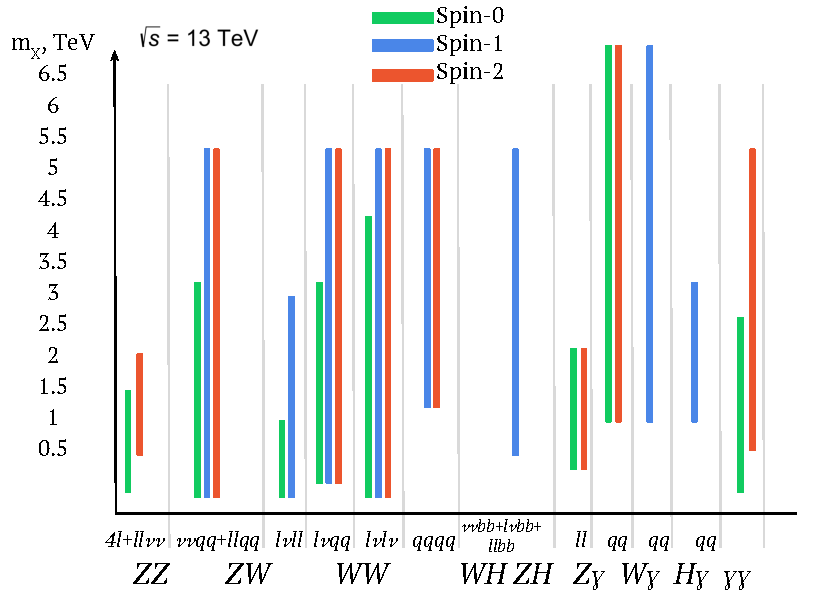
\includegraphics[width=.5\textwidth]{figures/lim_sketch}
     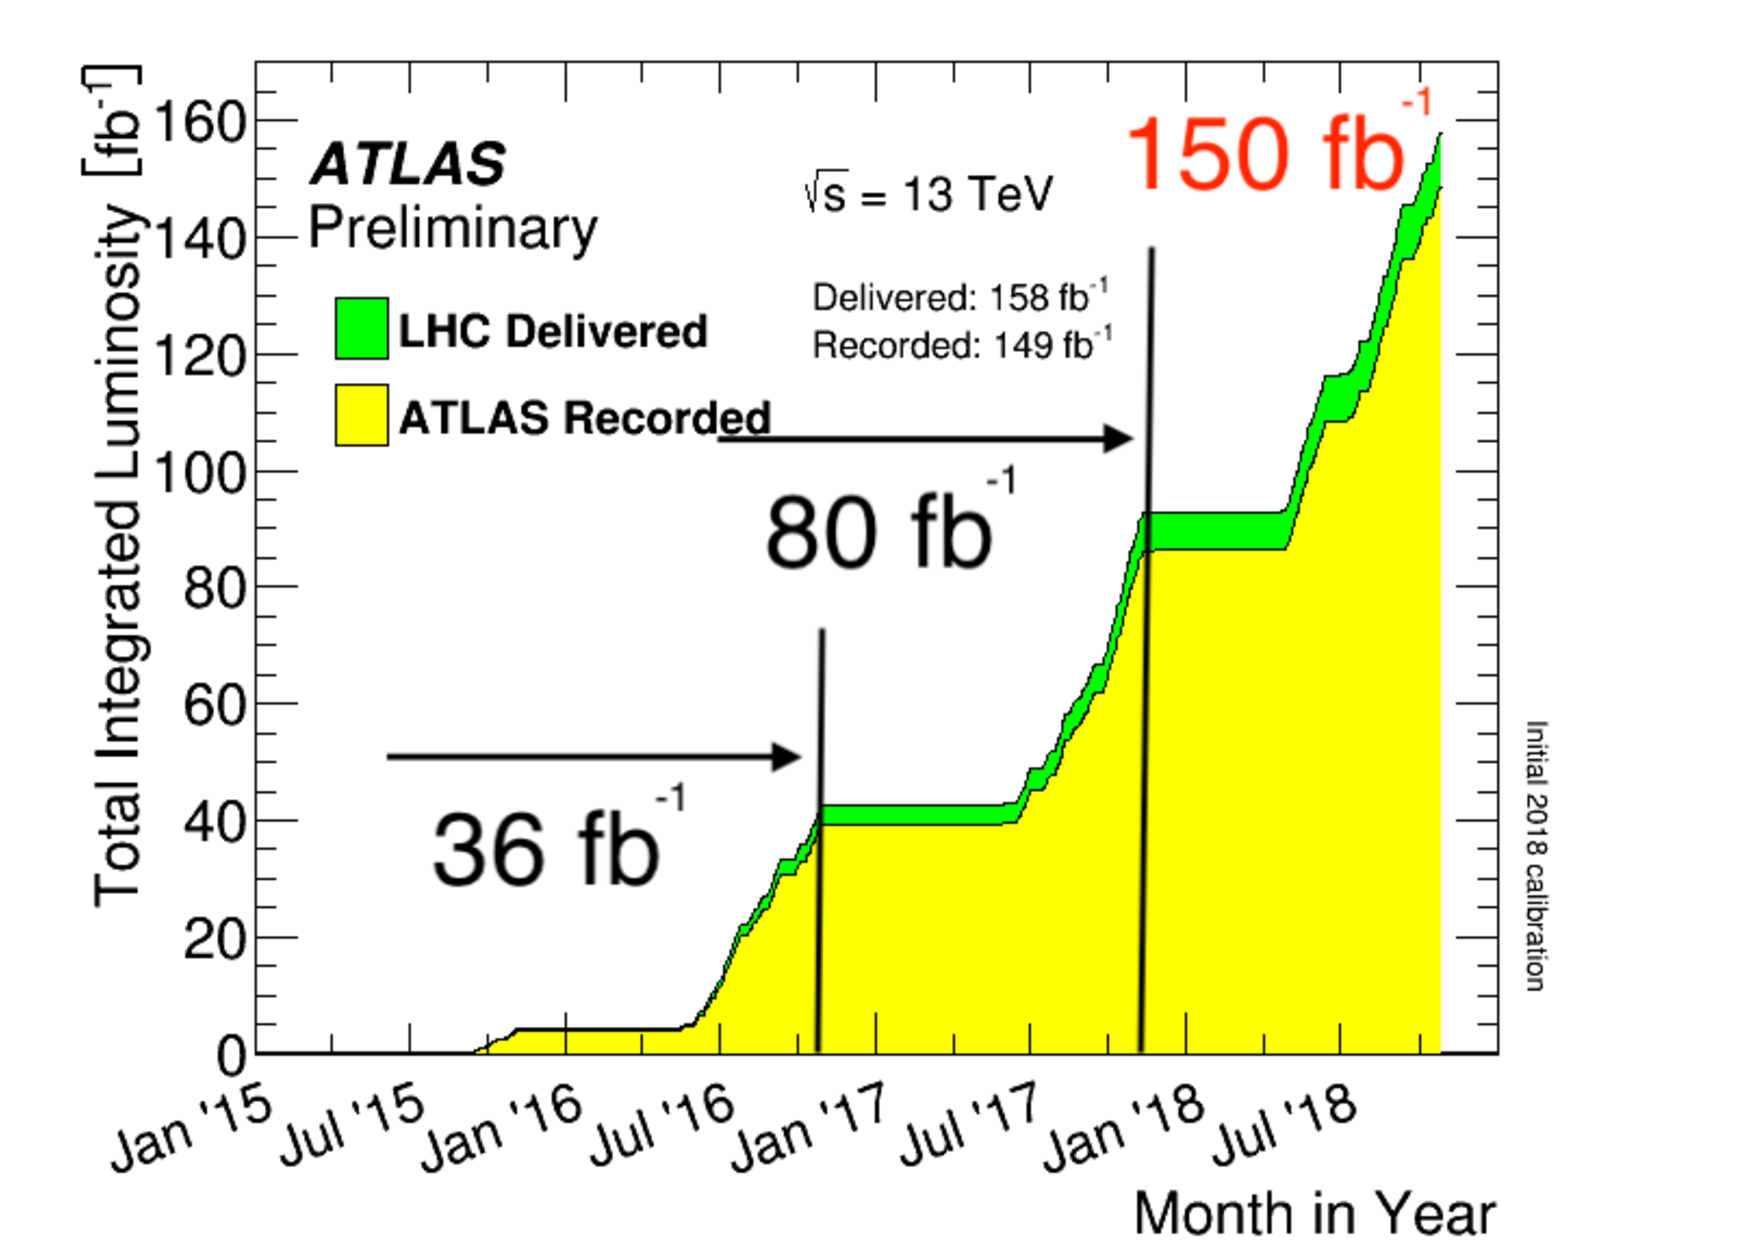
\includegraphics[width=.5\textwidth]{figures/intlumivstimeRun2}
     \caption{Left: combination of limits set on various diboson channels, covering large mass range and spin hypothesis. Right: cumulative luminosity versus time recorded by ATLAS (yellow).}
     \label{fig:summary}
     \end{figure}




%\printbibliography
\bibliographystyle{JHEP}

%\begin{thebibliography}{99}
\bibliography{all.bib}
%\bibliography{bib/CMS.bib}
%\bibitem{test}
%ATLAS collaboration, G. Aad et al., \textit{Observation of a new particle in the search for the Standard Model Higgs boson with the ATLAS detector at the LHC, Phys. Lett.} B716 (2012) 1-29, [1207.7214].
%%%
%\end{thebibliography}

\end{document}
